\chapter{Sensor Application}

\section{Health Sensors}
Hacking insulin pump~\cite{radcliffe2011hacking}
\section{Application}

\subsection{Initialization}
~\autoref{fig:init_ibe}
Every device should connect to mobile thorugh e.g. \gls{NFC} for initialization.
This results in a physical authentication between the device, and the mobile (i.e. the end user).
\begin{figure}[ht]
  \centering
  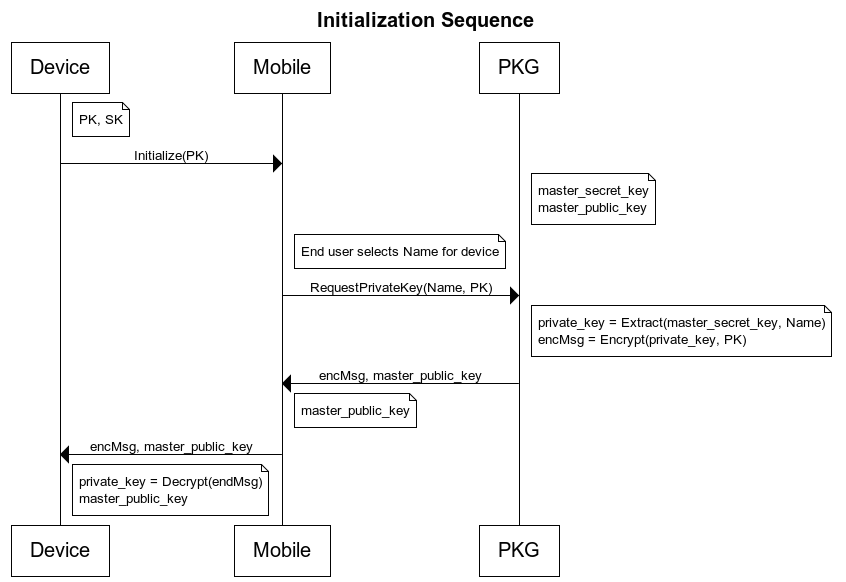
\includegraphics[width=1\textwidth]{init_ibe.png}
  \caption{Initialization IBE}
  \label{fig:init_ibe}
\end{figure}

% \begin{lstlisting}[language=BASH, caption={Initialization}, label={lst:ibe-initialization}]
% pkg = new PublicKeyGenerator;
% for device in {devices}
% do
% 	device -> connect to pkg;
% 	pkg -> verify device then issue Private Key;
% 	device -> subscribe Name Sync and Public Key
% done
% \end{lstlisting}


\subsection{Access Control}

\subsection{Public Key Infrastructure}

\subsection{Identity-Based Cryptography}